\documentclass[11pt]{article}
\usepackage[a4paper,margin=1in]{geometry}
\usepackage{amsmath,amssymb}
\usepackage{booktabs}
\usepackage{graphicx}
\usepackage{xcolor}
\usepackage{hyperref}
\hypersetup{colorlinks=true,linkcolor=blue,urlcolor=blue}

\newcommand{\rt}[1]{\texttt{#1}}
\providecommand{\ket}[1]{|#1\rangle}
\providecommand{\bra}[1]{\langle #1|}

\title{\textbf{Report R2 --- Unitary sweep and fragmentation scaling}\\
\large Krylov sector analysis of quantum cellular automata (Tier 1a/1c)}
\author{QCA Sector Analysis project (Tier 1)}
\date{2026-07-12 \quad\small(engine\_version \texttt{1a.1})}

\begin{document}
\maketitle

\begin{abstract}
We sweep all sixteen unitary quantum elementary cellular automata over chain
lengths $N=6\ldots18$, both boundary conventions, and classify each by the
scaling of its Krylov-sector structure. Sector sizes are exact; the growth of
the number of sectors and of the largest sector $D_{\max}$ is fit by BIC model
selection ($\ln y=c\,[+\alpha\ln N]\,[+\kappa N]$). Seven rules are effectively
ergodic under \rt{obc0} and nine under \rt{pbc}; that verdict originally rested
on $N=6$ alone, and \S\ref{sec:ergodic} re-establishes it over $N=6\ldots13$ with
the full sector decomposition, where it turns out to be exactly $N$-independent
and derivable from the rule encoding. The remaining rules fall into three
fragmentation families: exponential ($156/198$, $108$, $201$), a
domain-wall family with a linearly growing sector count but an extensive
$D_{\max}=2^{N-1}$ ($60/102$, \rt{obc0} only), and $150/105$ with central-binomial
sectors. We highlight two boundary-sensitive phenomena and one broken symmetry.
\end{abstract}

\section{Method}
Each unit $(\text{rule},N,\text{bc})$ is computed by the exact Tier-1a engine
(Report R1) and cached as one JSON line in \rt{results/}. Unitary sectors are the
weakly connected components of the one-cycle transition graph (extracted by
union--find; see R1). A rule is flagged \emph{effectively ergodic at $N$} when one
sector exceeds $90\%$ of the $2^N$ states; the sweep then stops increasing $N$ for
that rule/bc. Growth classes are assigned to the series $y(N)\in\{\#\text{sectors},
D_{\max}\}$ by BIC selection among constant / power-law / exponential models, with
the $\alpha\ln N$ prefactor always carried when reporting the exponential rate
$\kappa$ (so that $\sqrt N$-type binomial prefactors do not bias $\kappa$).

\section{Results}
Table~\ref{tab:summary} lists every computed rule/bc with its sector count and
$D_{\max}$ at the largest $N$ reached and the fitted growth classes. Figures
\ref{fig:nsec}--\ref{fig:scatter} show the scaling.

\begin{table}[h]
\centering
\small
\begin{tabular}{@{}rl l r rr l l@{}}
\toprule
W & tuple & bc & $N_{\max}$ & \#sec & $D_{\max}$ & \#sec growth & $D_{\max}$ growth (base) \\
\midrule
150 & \texttt{IVVI} & obc0 & 20 & 11 & 352716 & polynomial & exponential (2.022) \\
60 & \texttt{IIVV} & obc0 & 21 & 22 & 1048576 & polynomial & exponential (2.000) \\
102 & \texttt{IVIV} & obc0 & 21 & 22 & 1048576 & polynomial & exponential (2.000) \\
105 & \texttt{VIIV} & obc0 & 21 & 11 & 705432 & polynomial & exponential (1.984) \\
201 & \texttt{VIII} & obc0 & 21 & 97229 & 28657 & exponential & exponential (1.618) \\
108 & \texttt{IIIV} & obc0 & 21 & 170625 & 10946 & exponential & exponential (1.617) \\
156 & \texttt{IIVI} & obc0 & 21 & 28657 & 432 & exponential & exponential (1.292) \\
198 & \texttt{IVII} & obc0 & 21 & 28657 & 432 & exponential & exponential (1.292) \\
204 & \texttt{IIII} & obc0 & 21 & 2097152 & 1 & exponential & constant \\
51 & \texttt{VVVV} & obc0$^{\dagger6}$ & -- & -- & -- & ergodic & ergodic \\
54 & \texttt{IVVV} & obc0$^{\dagger6}$ & -- & -- & -- & ergodic & ergodic \\
57 & \texttt{VIVV} & obc0$^{\dagger6}$ & -- & -- & -- & ergodic & ergodic \\
99 & \texttt{VVIV} & obc0$^{\dagger6}$ & -- & -- & -- & ergodic & ergodic \\
147 & \texttt{VVVI} & obc0$^{\dagger6}$ & -- & -- & -- & ergodic & ergodic \\
153 & \texttt{VIVI} & obc0$^{\dagger6}$ & -- & -- & -- & ergodic & ergodic \\
195 & \texttt{VVII} & obc0$^{\dagger6}$ & -- & -- & -- & ergodic & ergodic \\
105 & \texttt{VIIV} & pbc & 20 & 13 & 369512 & constant & exponential (1.994) \\
150 & \texttt{IVVI} & pbc & 20 & 13 & 369512 & polynomial & exponential (1.940) \\
108 & \texttt{IIIV} & pbc & 21 & 134643 & 24476 & exponential & exponential (1.619) \\
201 & \texttt{VIII} & pbc & 21 & 134643 & 24476 & exponential & exponential (1.619) \\
156 & \texttt{IIVI} & pbc & 21 & 24477 & 324 & exponential & exponential (1.301) \\
198 & \texttt{IVII} & pbc & 21 & 24477 & 324 & exponential & exponential (1.301) \\
204 & \texttt{IIII} & pbc & 21 & 2097152 & 1 & exponential & constant \\
51 & \texttt{VVVV} & pbc$^{\dagger6}$ & -- & -- & -- & ergodic & ergodic \\
54 & \texttt{IVVV} & pbc$^{\dagger6}$ & -- & -- & -- & ergodic & ergodic \\
57 & \texttt{VIVV} & pbc$^{\dagger6}$ & -- & -- & -- & ergodic & ergodic \\
60 & \texttt{IIVV} & pbc$^{\dagger6}$ & -- & -- & -- & ergodic & ergodic \\
99 & \texttt{VVIV} & pbc$^{\dagger6}$ & -- & -- & -- & ergodic & ergodic \\
102 & \texttt{IVIV} & pbc$^{\dagger6}$ & -- & -- & -- & ergodic & ergodic \\
147 & \texttt{VVVI} & pbc$^{\dagger6}$ & -- & -- & -- & ergodic & ergodic \\
153 & \texttt{VIVI} & pbc$^{\dagger6}$ & -- & -- & -- & ergodic & ergodic \\
195 & \texttt{VVII} & pbc$^{\dagger6}$ & -- & -- & -- & ergodic & ergodic \\
\bottomrule
\end{tabular}

\caption{Per-rule fragmentation scaling (unitary rules). $^{\dagger}N$ marks the
$N$ at which a rule first becomes effectively ergodic for that boundary
convention. Rules reduced by reflection are represented once where noted.}
\label{tab:summary}
\end{table}

\begin{figure}[h]
\centering
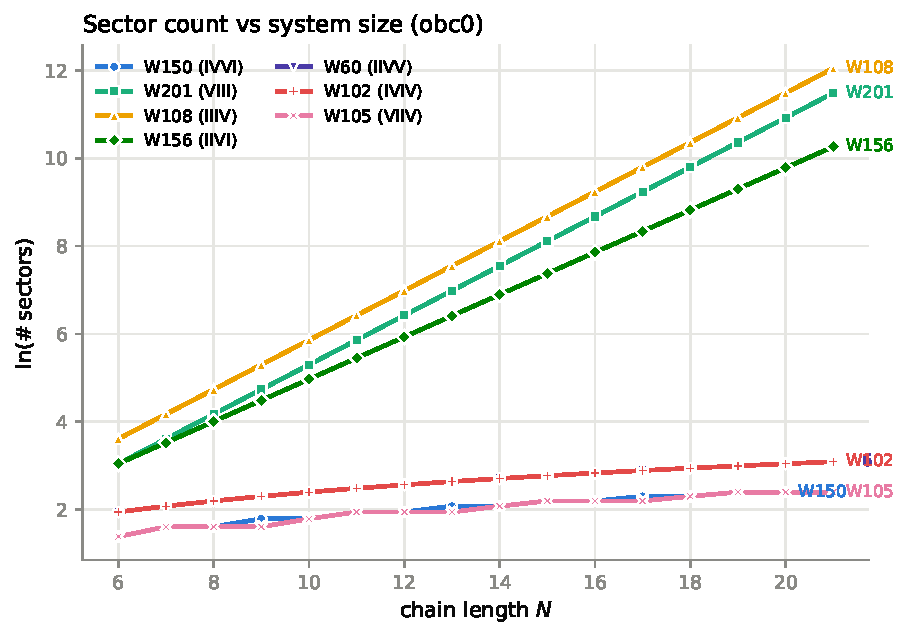
\includegraphics[width=0.78\linewidth]{../../figures/fig_nsectors_obc0.pdf}
\caption{Number of Krylov sectors vs $N$ (\rt{obc0}), log scale. Exponential
fragmentation ($156$, $108$, $201$) vs.\ linear/central-binomial sector counts
($60/102$, $150/105$).}
\label{fig:nsec}
\end{figure}

\begin{figure}[h]
\centering
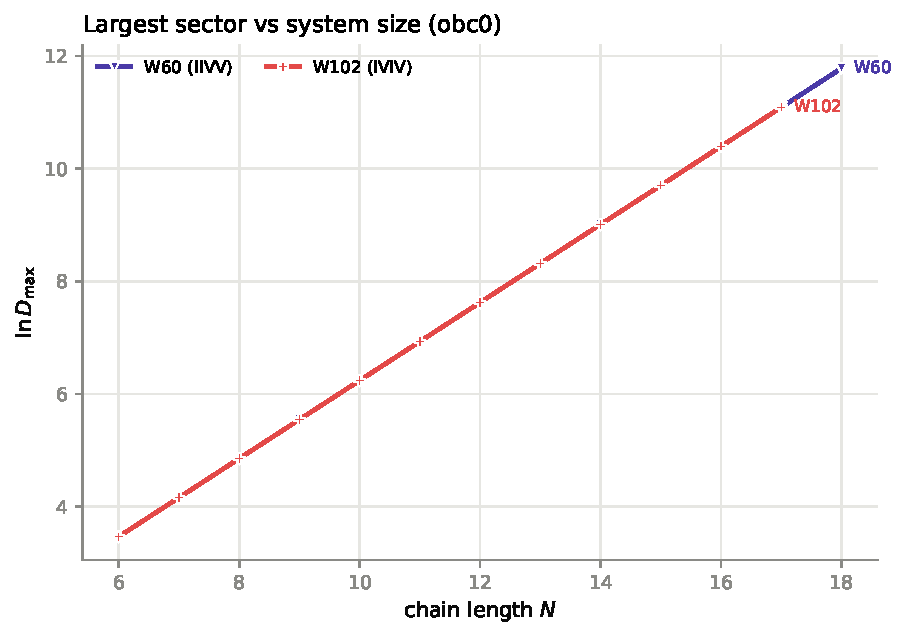
\includegraphics[width=0.78\linewidth]{../../figures/fig_dmax_obc0.pdf}
\caption{Largest sector $D_{\max}$ vs $N$ (\rt{obc0}), log scale. Slopes give the
exponential base: $\varphi$ (golden ratio) for $201$, $4^{1/5}\approx1.3195$ for
$156/198$, $2$ for the domain-wall family $60/102$.}
\label{fig:dmax}
\end{figure}

\begin{figure}[h]
\centering
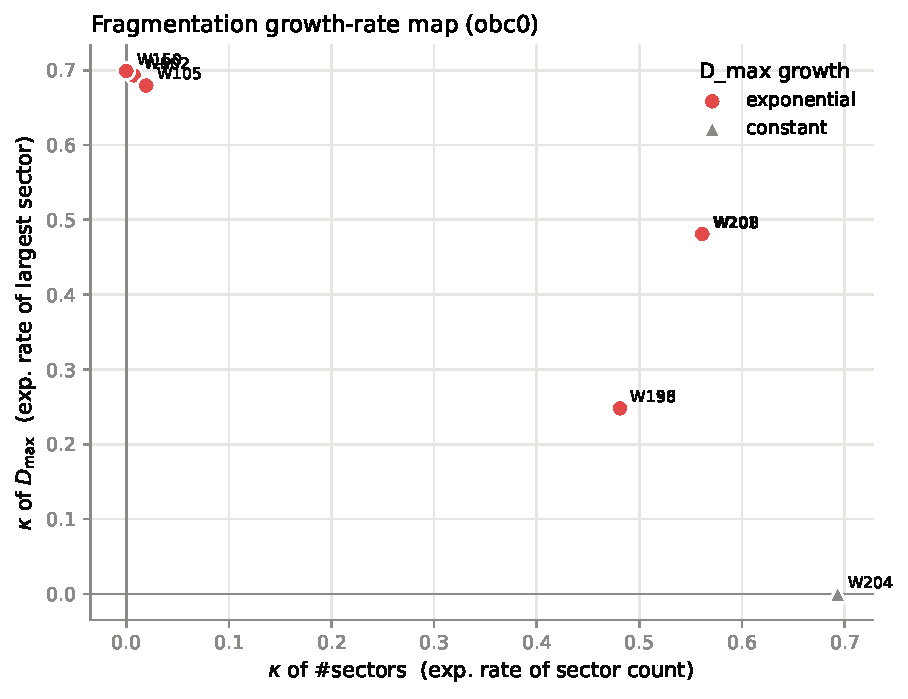
\includegraphics[width=0.72\linewidth]{../../figures/fig_growth_scatter_obc0.pdf}
\caption{Growth-\emph{base} map (\rt{obc0}): the base $b=e^{\kappa}$ of the
sector count against that of the largest sector, one point per rule. Plotting
$b\in[1,2]$ rather than $\kappa\in[0,\ln 2]$ puts the named constants at
recognisable positions; the dotted lines mark them. $\dagger$ marks a base from
the two-parameter fit $\ln y=c+\kappa N$ rather than an exact recurrence --- note
in particular that the M2 model $c+\alpha\ln N+\kappa N$ used for the growth
\emph{class} is biased low as a rate estimator, reporting $1.281$ for $156/198$
against its true asymptote $4^{1/5}$.}
\label{fig:scatter}
\end{figure}

\section{A caution on reading bases off these fits: rule 156}
\label{sec:156}
The growth-base map invites reading a constant off each point, and $156/198$ is
the case where that fails. Its $D_{\max}$ series (\rt{obc0}) is
\[
  6,\,9,\,12,\,16,\,20,\,27,\,36,\,48,\,64,\,81,\,108,\,144,\,192
  \qquad (N=6\ldots18),
\]
and it satisfies \emph{both} $a(N{+}4)=3a(N)$ and $a(N{+}5)=4a(N)$ with exactly
the same two exceptions ($N=6,10$). The implied bases are $3^{1/4}=1.31607$ and
$4^{1/5}=1.31951$ --- they differ by $0.26\%$, and thirteen terms cannot choose
between them. No fit should be allowed to.

The combinatorial derivation does choose. Writing the chain as ``rooms'' of
length $l$ separated by domain walls, a room contributes $l+1$ states and
consumes $l+2$ sites, so $D_{\max}=b^N$ with
\begin{equation}
  b(l)=(l+1)^{1/(l+2)} ,
\end{equation}
whose saddle point $\mathrm{d}\ln b/\mathrm{d}l=0$ gives the transcendental
condition $\ln x = 1+1/x$ with $x=l+1$, i.e.\ $l\approx 2.5911$. The two
integer neighbours of that optimum are precisely the two candidates above, and
$l=3$ is the larger:
\[
  b(2)=3^{1/4}=1.31607 \;<\; b(3)=4^{1/5}=1.31951 .
\]
So the asymptotic base is $4^{1/5}$, and at finite $N$ the largest sector is a
\emph{mixture} of rooms of length 2 and 3 --- which is exactly why neither pure
recurrence is exact over the computed range. This is the one base in the report
that comes from theory rather than from the data, and it should stay that way.

A second, purely numerical trap sits on the same rule. The BIC model
$\ln y = c+\alpha\ln N+\kappa N$ is the right tool for the growth \emph{class},
but its $\alpha\ln N$ term absorbs part of the growth and makes $\kappa$ a
biased rate estimator: it reports base $1.281$ for $156/198$, far enough below
$4^{1/5}$ to look like a different constant. Rates in the growth-base map are
therefore taken from the two-parameter fit $\ln y=c+\kappa N$, or from an exact
recurrence where one exists.

\section{The ergodic rules are ergodic at every $N$, not just at $N=6$}
\label{sec:ergodic}
The ergodicity verdict as originally produced rested on a single system size.
The sweep aborts a unit the moment one component exceeds $90\%$ of $2^N$ and then
stops increasing $N$ for that rule, so an ergodic-flagged unit had exactly one
record, at $N=6$ --- and it carried no sector data at all, only the flag. Six
sites is far too small to distinguish genuine ergodicity from a finite-size
accident, so this claim was re-established from scratch: every ergodic-flagged
unit was recomputed with the abort disabled (\rt{run\_rule -{}-no-ergodic-abort}),
which performs the \emph{full} decomposition and reports how many sectors there
really are, over $N=6\ldots13$.

The outcome is completely rigid. Across all sixteen units and all eight sizes,
only two structures occur --- one sector of size $2^N$, or one sector of size
$2^N-1$ together with a single frozen basis state --- and \emph{each unit gives
the same structure at every $N$}. Nothing drifts, nothing crosses over, and no
small sector appears at any size.

\begin{center}\small
\begin{tabular}{llll}
\toprule
rule & tuple & \rt{pbc} & \rt{obc0}\\
\midrule
$51$  & $\rt{VVVV}$ & $\{2^N\}$ & $\{2^N\}$\\
$57$  & $\rt{VIVV}$ & $\{2^N\}$ & $\{2^N\}$\\
$99$  & $\rt{VVIV}$ & $\{2^N\}$ & $\{2^N\}$\\
$54$  & $\rt{IVVV}$ & $\{2^N\!-\!1,\,1\}$ & $\{2^N\!-\!1,\,1\}$\\
$60$  & $\rt{IIVV}$ & $\{2^N\!-\!1,\,1\}$ & fragmented ($N+1$ sectors)\\
$102$ & $\rt{IVIV}$ & $\{2^N\!-\!1,\,1\}$ & fragmented ($N+1$ sectors)\\
$147$ & $\rt{VVVI}$ & $\{2^N\!-\!1,\,1\}$ & $\{2^N\}$\\
$153$ & $\rt{VIVI}$ & $\{2^N\!-\!1,\,1\}$ & $\{2^N\}$\\
$195$ & $\rt{VVII}$ & $\{2^N\!-\!1,\,1\}$ & $\{2^N\}$\\
\bottomrule
\end{tabular}
\end{center}

The pattern is not empirical --- it follows from the encoding, which is why more
data would add nothing. The all-zeros state has every site sitting in neighbour
configuration $(0,0)$, so it is frozen precisely when $r_{00}=\rt I$; the
all-ones state has every site in configuration $(1,1)$ and is frozen precisely
when $r_{11}=\rt I$. Those are the only two configurations that are homogeneous
across the whole chain, so no other singleton sector can exist. The table follows
immediately: $54/60/102$ carry $r_{00}=\rt I$ and freeze the vacuum under both
conventions; $147/153/195$ carry $r_{11}=\rt I$ and freeze $\ket{1\cdots1}$ under
\rt{pbc} only, because the \rt{obc0} padding gives the two end sites a $0$
neighbour and breaks the homogeneity; $51/57/99$ have neither and are a single
sector. The singleton was verified directly at $N=8$ in each case.

The practical upshot for the scaling tables is that these units are not missing
data but a trivial growth law: $\#\text{sectors}$ is constant ($1$ or $2$) and
$D_{\max}=2^N$ or $2^N-1$, i.e.\ exponential with base exactly $2$.

\section{Boundary-sensitive fragmentation}
Two rules change fragmentation class with the boundary:
\begin{itemize}
  \item \textbf{Rules 60/102 $(\rt{IIVV})/(\rt{IVIV})$:} under \rt{obc0} the
  domain-wall charge fragments the space into $N+1$ sectors with an extensive
  dominant sector $D_{\max}=2^{N-1}$; under \rt{pbc} the periodic seam destroys
  the charge and the dynamics is ergodic --- a single sector of size $2^N-1$ plus
  the frozen vacuum $|0\cdots0\rangle$ ($D_{\max}/2^N\to1$).
  \item \textbf{Rules 150/105:} identical sector data under \rt{obc0} (central
  binomials $\binom{N+1}{w}$), but they \emph{differ} under \rt{pbc}, where the
  periodic domain-wall counting is rule-specific.
\end{itemize}

\section{Broken inversion symmetry (201 vs.\ 108)}
Rules $201=(\rt{VIII})$ and $108=(\rt{IIIV})$ are $0\!\leftrightarrow\!1$
spin-flip partners. Because the flip conjugates the Hadamard by $X$ and
$XHX\neq\pm H$, the symmetry is broken for the full dynamics. At the level of the
sector partition it survives under \rt{pbc} (bit-flip is a graph symmetry: $|XHX|
=|H|$) but is broken under \rt{obc0} by the vacuum-0 padding: there $201$ has
Fibonacci $D_{\max}$ and $108$ shifted-Fibonacci $D_{\max}$ (matching \rt{HSF}
rules 1 and 8). See Report R1 for the exact statement.

\section{Reproducibility}
All numbers derive from \rt{results/*.jsonl} (engine\_version \texttt{1a.1});
the table and figures are regenerated by
\rt{python -m qca\_fragmentation.scaling.summary} and
\rt{...scaling.figure}. The sweep is idempotent and checkpointed
(\rt{checkpoints/manifest.jsonl}).

\end{document}
